% nano-AgentRL report skeleton (arXiv style, single column).
% Build: pdflatex main && bibtex main && pdflatex main && pdflatex main
% Every \todo{} marks a number or claim that must come from a real run.
\documentclass[11pt]{article}
\usepackage[margin=1in]{geometry}
\usepackage[T1]{fontenc}
\usepackage{lmodern}
\usepackage{amsmath,amssymb}
\usepackage{booktabs}
\usepackage{graphicx}
\usepackage{xcolor}
\usepackage[hidelinks]{hyperref}
\usepackage[numbers]{natbib}

\newcommand{\todo}[1]{\textcolor{red}{\textbf{[TODO: #1]}}}
\graphicspath{{../docs/figures/}}

\title{nano-AgentRL: Does RL Make Search Agents Reliable, or Only Accurate?}
\author{Prince}
\date{October 2026}

\begin{document}
\maketitle

\begin{abstract}
We re-implement Search-R1~\cite{jin2025searchr1} from scratch: multi-turn
GRPO~\cite{shao2024deepseekmath} with retrieved-token loss masking, about 1{,}600 lines of
PyTorch, trained end to end on one free 2$\times$T4 Kaggle notebook. On 500 NQ and 500
HotpotQA questions the agent reaches 13.0 and 19.6 exact match, from 0.2 and 0.4 for the
untrained model. We then ask a question accuracy alone cannot answer: does the trained agent
succeed \emph{consistently}? Sampling eight responses per question, pass@8 is 21--28\% but
pass$^8$ is 0--4\%: the agent solves a quarter of the questions \emph{sometimes}, and almost
none \emph{every time}. A rule-based failure taxonomy attributes about 70\% of failures to
retrieval, so the consistency ceiling is set by the retriever and by the queries the policy
writes, not by decoding noise alone.
\end{abstract}

\section{Introduction}
An agent is deployed where a single failure is expensive: a wrong refund, a missed
contraindication, a broken migration. Aggregate accuracy hides this, because a model that
succeeds half the time on every question looks identical to one that succeeds on half the
questions every time. The difference is what pass$^k$~\cite{yao2024taubench} measures: the
probability that \emph{all} $k$ samples of the same question are correct.

This report asks whether RL training on a search agent buys consistency or only accuracy.
We contribute:
(1) a minimal, readable GRPO trainer for multi-turn search agents, about 1{,}600 lines of
PyTorch, no verl and no TRL in the training loop, with 178 CPU tests;
(2) a reproduction of Search-R1 on hardware anyone can use for free, one 2$\times$T4 Kaggle
notebook for 2.9 hours;
(3) a reliability analysis across training, where capability and consistency move apart, and
a failure taxonomy that localises the gap to retrieval.

\section{Background}
\subsection{GRPO}
For each question $q$, sample $G$ responses $o_1,\dots,o_G$ with rewards $r_i$. The advantage
of every token of $o_i$ is
\begin{equation}
  A_i = \frac{r_i - \operatorname{mean}(r)}{\operatorname{std}(r) + \epsilon}.
\end{equation}
With ratio $\rho_{i,t} = \pi_\theta(o_{i,t}\mid q,o_{i,<t}) / \pi_{\text{old}}(o_{i,t}\mid q,o_{i,<t})$,
the per-token objective is
\begin{equation}
  \min\!\big(\rho_{i,t} A_i,\ \operatorname{clip}(\rho_{i,t}, 1-\varepsilon, 1+\varepsilon) A_i\big)
  - \beta\, \mathbb{D}_{\text{KL}}^{k3}\!\left[\pi_\theta \,\|\, \pi_{\text{ref}}\right],
\end{equation}
with the k3 estimator $e^{x} - x - 1$, $x = \log \pi_{\text{ref}} - \log \pi_\theta$~\cite{shao2024deepseekmath}.
Dr.~GRPO~\cite{liu2025drgrpo} removes the std normalization and the per-sequence length normalization.

\subsection{Search-R1}
The model interleaves \texttt{<think>}, \texttt{<search>} and \texttt{<answer>}. Retrieved
documents are appended inside \texttt{<information>} and excluded from the loss.

\subsection{Reliability metrics}
For $n$ samples with $c$ correct, $\text{pass@}k = 1 - \binom{n-c}{k}/\binom{n}{k}$~\cite{chen2021codex}
and $\text{pass}^k = \binom{c}{k}/\binom{n}{k}$~\cite{yao2024taubench}.

\section{Implementation}
The trainer is organised as a pipeline of small modules --- log-probs, GRPO, rollouts, trainer,
generation, rewards --- each paired with a deliberately slow reference implementation in the
tests. Master weights stay in float32 while the forward pass runs under bf16 autocast: pure
bf16 weights silently drop updates of size $\mathrm{lr}\cdot g \sim 10^{-6}$ on weights of
order $10^{-2}$, which looks like a flat loss curve rather than a bug. Rollouts are split into
micro-batches whose gradients are summed exactly under every supported loss aggregation, and
a test asserts that the result matches a single full batch. Generation uses HF
\texttt{generate} on the T4 notebook and vLLM when available, copying the updated policy into
the engine after each step. A token-level mask removes retrieved documents from the loss, so
the gradient covers only tokens the model produced.

\section{Reproduction}
Setup: Qwen2.5-0.5B-Instruct, group size 8, two turns, 300 generated tokens per turn, BM25
top-3 over the 21M-passage wiki-18 corpus, 90 optimizer steps. Training took 2.9 hours on a
free Kaggle 2$\times$T4 notebook; every cell of that run is reproducible from the repository's
notebook. Rows 1--2 are measured with the same harness, retrieval disabled or with the
question as the only query.
\begin{table}[h]
\centering
\begin{tabular}{lcccc}
\toprule
Method (Qwen2.5-0.5B-Instruct) & NQ EM & NQ gold-in-ans. & HotpotQA EM & HotpotQA gold-in-ans. \\
\midrule
Direct (no retrieval)  & 0.2 & 13.2 & 0.4 & 17.2 \\
RAG (one retrieval)    & 0.0 & 22.0 & 0.8 & 27.4 \\
Ours, GRPO 90 steps    & \textbf{13.0} & 16.0 & \textbf{19.6} & 25.4 \\
\bottomrule
\end{tabular}
\caption{500 NQ + 500 HotpotQA questions (dev\_500 subsets), greedy, BM25 top-3. Gold-in-answer:
a gold answer appears anywhere in the model's own text. GSM8K (single-turn GRPO, 200 steps):
32.4 $\to$ 47.9 EM on the full test set. \todo{3B results on an 80\,GB GPU; Search-R1 paper
numbers for reference}}
\end{table}

Two observations matter for the rest of the paper. First, strict EM moves from roughly zero to
13--20 while invalid outputs fall from 99\% to under 1\%: most of the visible gain is the model
learning to \emph{state} an answer in the required format. Second, on the lenient
gold-in-answer metric the agent does \emph{not} beat single-step RAG (25.4 vs 27.4 on
HotpotQA). The policy was not learning to find more answers; it was learning to commit to one.

\begin{figure}[h]
\centering
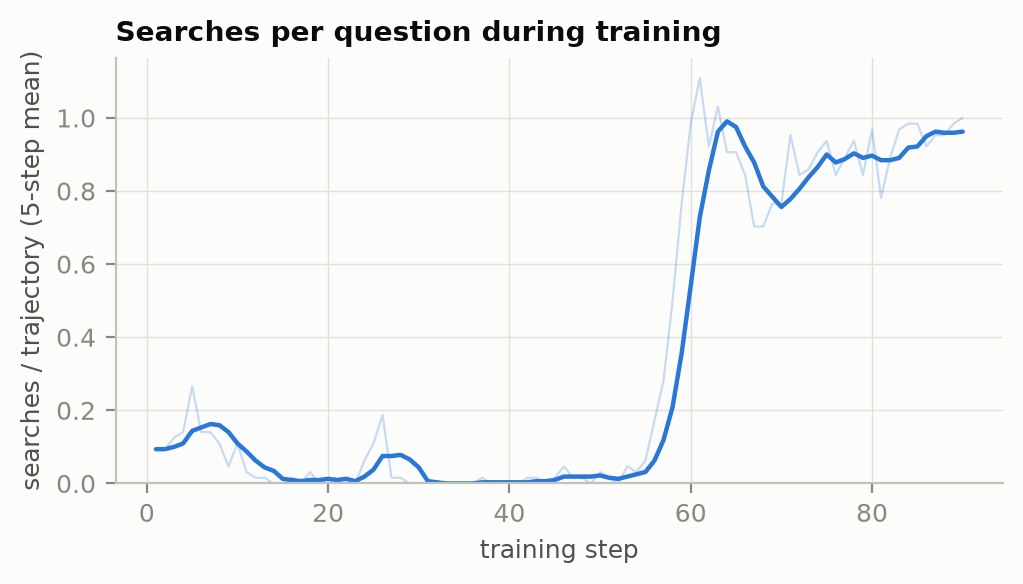
\includegraphics[width=0.7\linewidth]{search_0.5b_t4/fig4_searches.png}
\caption{Searches per trajectory during search training: a format shortcut (steps 10--55),
then abrupt discovery of retrieval around step 56.}
\end{figure}

\section{Reliability Analysis}
We sample 8 responses per question at temperature 1.0 on 100-question subsets, at the last two
checkpoints (steps 75 and 90), and score every trajectory with the rule judge. Table~\ref{tab:reliability}
reports capability (pass@$k$: \emph{at least one} of $k$ correct) next to consistency
(pass$^k$: \emph{all} $k$ correct).

\begin{table}[h]
\centering
\begin{tabular}{lcccccc}
\toprule
& & \multicolumn{2}{c}{capability} & \multicolumn{2}{c}{consistency} & \\
\cmidrule(lr){3-4}\cmidrule(lr){5-6}
Split & step & pass@1 & pass@8 & pass$^4$ & pass$^8$ & searches \\
\midrule
NQ       & 75 & 7.8  & 21 & 1.1 & 0.0 & 0.90 \\
NQ       & 90 & 8.6  & 21 & 3.5 & 3.0 & 0.98 \\
HotpotQA & 75 & 10.5 & 27 & 3.0 & 1.0 & 0.90 \\
HotpotQA & 90 & 14.1 & 28 & 5.9 & 4.0 & 0.98 \\
\bottomrule
\end{tabular}
\caption{Capability and consistency at the last two checkpoints (percent, 100 questions per
split, 8 samples, temperature 1.0). ``Searches'' is mean search calls per trajectory.}
\label{tab:reliability}
\end{table}

\begin{figure}[h]
\centering
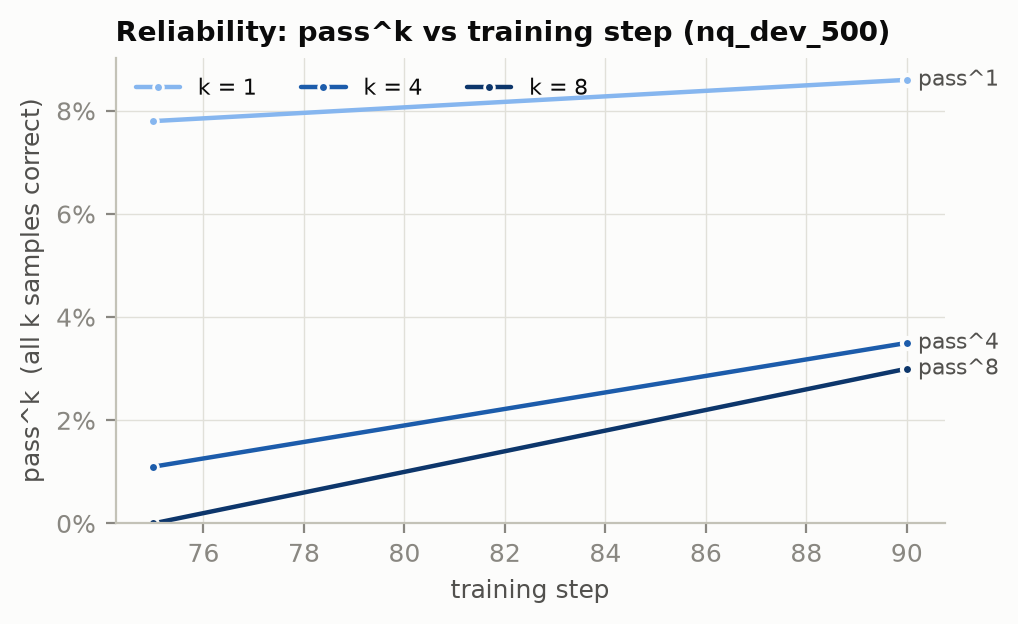
\includegraphics[width=0.48\linewidth]{search_0.5b_t4/reliability_nq_dev_500/fig2_pass_hat_k.png}\hfill
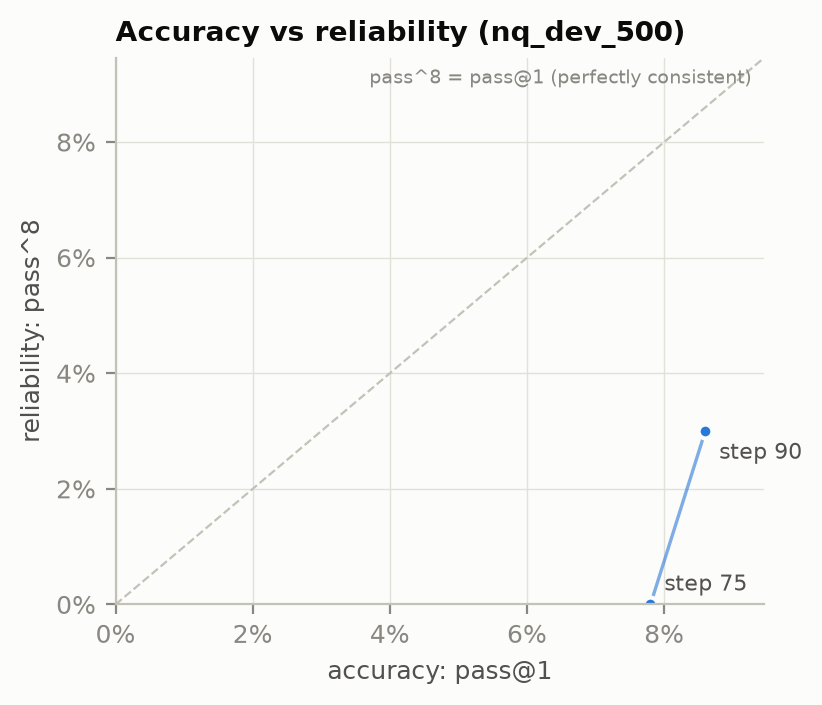
\includegraphics[width=0.40\linewidth]{search_0.5b_t4/reliability_nq_dev_500/fig3_acc_vs_reliability.png}
\caption{Left: pass$^k$ for $k \in \{1,2,4,8\}$ over training (NQ). Right: accuracy vs
reliability; the dashed line is perfect consistency. Every checkpoint sits far below it.}
\end{figure}

\begin{figure}[h]
\centering
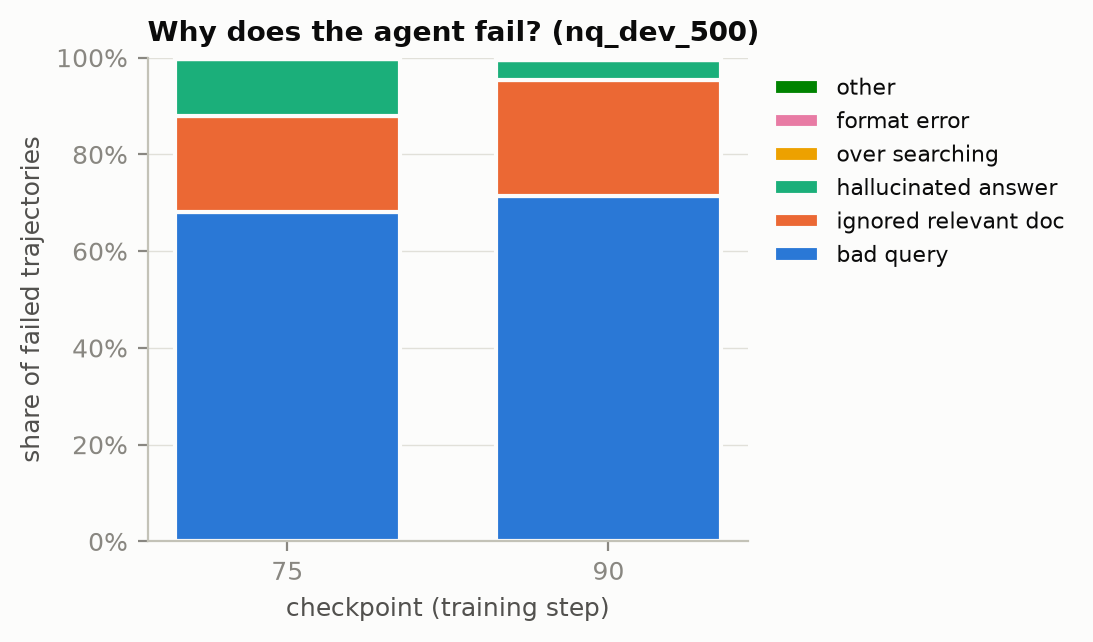
\includegraphics[width=0.6\linewidth]{search_0.5b_t4/reliability_nq_dev_500/fig5_failure_taxonomy.png}
\caption{Failure taxonomy per checkpoint (NQ). ``Bad query'' covers any failure where the gold
passage never reached the context, which implicates BM25 and the corpus as well as the policy.
Judge agreement with 50 hand labels: \todo{accuracy, $\kappa$}.}
\end{figure}

Four findings:
\begin{enumerate}
\item \textbf{Capability far exceeds consistency.} pass@8 is 21--28\%: the agent can answer a
quarter of the questions \emph{sometimes}. pass$^8$ is 0--4\%: almost none \emph{every time}.
The gap is 18--24 points, so most solvable questions are coin flips.
\item \textbf{Late training buys consistency faster than accuracy.} From step 75 to 90 pass@1
rose 1--4 points while pass$^4$ and pass$^8$ grew 2--4$\times$ from a small base. pass@8 did
not move: the agent is not reaching new questions, it is becoming more repeatable on the ones
it could already solve.
\item \textbf{pass@8 tracks one-shot RAG.} NQ 21 vs 22, HotpotQA 28 vs 27.4 (Table~1). Sampling
eight times recovers roughly what a single RAG generation already \emph{contains}, which points
at the retrieval ceiling rather than the decoding budget.
\item \textbf{Most failures are retrieval failures.} About 70\% of failures are ``bad query'':
the gold never appeared in the retrieved passages. A further 19--24\% are reading failures,
where the gold was in the context and the agent answered something else. Answering without
searching fell from 12\% to 4\% of failures between the two checkpoints.
\end{enumerate}

These findings motivate a measurement the repository now ships but has not yet run at scale:
recall@3 of the raw question versus the query the policy writes
(\texttt{scripts/retrieval\_recall.py}). If the policy's query retrieves the gold less often
than the question does, consistency is limited by the search behaviour; if both are low, BM25
or the corpus is the ceiling.

\section{Limitations}
Two checkpoints, one seed, and 100 questions per split (pass@1 is $\pm$1--2 points with 8
samples). The taxonomy uses a rule judge that has not yet been validated against hand labels.
BM25 rather than a trained retriever, 500-question dev subsets rather than full test sets, and
0.5B parameters only.

\section{Ablations}
Planned, not yet run: baseline, no loss mask, Dr.~GRPO, $G=4$ vs $G=8$, base vs instruct;
final EM and pass$^8$ with 3 seeds. \todo{run these; they need the 80\,GB GPU}

\section*{Availability}
Code, figures and the runnable Kaggle notebook:
\url{https://github.com/PRINCE2-AI/nano-agentrl}. A shorter version of this analysis is
published at
\url{https://thereliableagent.substack.com/p/pass8-was-28-pass8-was-4-same-model}.

\bibliographystyle{plainnat}
\bibliography{refs}
\end{document}
